\documentclass{vldb}

%% Language and font encodings
 %\usepackage[english]{babel}
\usepackage[utf8x]{inputenc}
\usepackage[T1]{fontenc}
% \usepackage{amsthm}
\usepackage{paralist}
\usepackage[ruled, vlined]{algorithm2e}

\usepackage{amsmath}
\usepackage{graphicx}
\usepackage{accents}
\usepackage{diagbox}
\usepackage[colorinlistoftodos]{todonotes}
\usepackage{mathrsfs}
% \usepackage{hyperref}
\usepackage{subfig}
\usepackage{listings}
\usepackage{xparse}
\usepackage[super]{nth}
\usepackage{hyperref,cleveref}

\makeatletter
\DeclareRobustCommand{\cev}[1]{%
  \mathpalette\do@cev{#1}%
}
\newcommand{\do@cev}[2]{%
  \fix@cev{#1}{+}%
  \reflectbox{$\m@th#1\vec{\reflectbox{$\fix@cev{#1}{-}\m@th#1#2\fix@cev{#1}{+}$}}$}%
  \fix@cev{#1}{-}%
}
\newcommand{\fix@cev}[2]{%
  \ifx#1\displaystyle
    \mkern#23mu
  \else
    \ifx#1\textstyle
      \mkern#23mu
    \else
      \ifx#1\scriptstyle
        \mkern#22mu
      \else
        \mkern#22mu
      \fi
    \fi
  \fi
}

\newcommand{\forrest}[0]{\textsc{Forrest}\xspace}

\makeatother

\DeclareMathOperator*{\argmin}{argmin}
\DeclareMathOperator*{\argmax}{argmax}
\DeclareMathOperator*{\minimize}{minimize}
\DeclareMathOperator*{\maximize}{matximize}

\vldbTitle{FORREST: A Benchmarking Framework for Evaluating Tree~Matching Algorithms at~Scale}
\vldbAuthors{Ben Trovato, G. K. M. Tobin, Lars Th{\sf{\o}}rv{$\ddot{\mbox{a}}$}ld, Lawrence P. Leipuner, Sean Fogarty, Charles Palmer, John Smith, Julius P.~Kumquat, and Ahmet Sacan}
\vldbDOI{https://doi.org/10.14778/xxxxxxx.xxxxxxx}
\vldbVolume{12}
\vldbNumber{xxx}
\vldbYear{2019}


\begin{document}

% \theoremstyle{definition}
\newtheorem{defn}{Definition}[section]
\newtheorem{prop}{Property}[section]

% \theoremstyle{definition}
\newtheorem{assumption}{Assumption}[section]
\newtheorem{theorem}{Theorem}

% \theoremstyle{definition}
\newtheorem{rqn}{RQ}[section]

% \theoremstyle{definition}
\newtheorem{ex}{Example}[section]

% \theoremstyle{definition}
\newtheorem{note}{Note}[section]

\SetKw{Break}{break}
\SetKw{Continue}{continue}

\title{FORREST: A Benchmarking~Framework to~Evaluate Tree~Matching~Algorithms at~Large}

\maketitle

\begin{abstract}
Tree matching techniques have been investigated in many fields, including web data mining and extraction, as a key component to analyze the content of web documents.
However, state-of-the-art approaches, like \emph{Tree-Edit Distance} (TED) and its variants, fail to scale beyond a few hundreds of nodes, which is far below the average complexity of existing web online documents and applications.

%In this paper, we therefore propose a novel similarity-based FTM algorithm that proposes a similarity metric to scale beyond the current limits.
In this paper, we therefore propose\dots
\end{abstract}

\section{Introduction} 
% What is tree matching
Comparing trees is at the core of several different research challenges in a wide variety of fields from software static analysis, to computational biology.
To compare two trees, computing a distance metric between them is sometimes sufficient but, in many situations, applications require more precise one-to-one associations between the nodes of both trees.
Computing this mapping between source and destination nodes is called \textit{tree matching}.

% How tree matching is done
The classic approach to \textit{tree matching} is \textit{Tree Edit Distance} (TED).
The tree edit distance between two trees $t$ and $t'$ is defined as the least-cost sequence of edit operations that transforms $t$ into $t'$.
By definition, TED imposes two significant restrictions to the general tree matching problem: the order of ancestors and the order of siblings between the two trees compared must be preserved.
These constraints allow TED to produce optimal matching in tractable times.
Without enforcing these constraints, finding the optimal solution to the tree matching problem has been shown to be NP-hard. 

% The limits of the current approach
However, the constraints to the general tree matching imposed by TED can be very problematic in some situations~\cite{Kumar2011_FTM, reis2004automatic}.
Yet, at the time of writing this paper, almost all seminal works offering a tree matching solution formally derive from TED, either to improve on its implementation or to improve the computation speed by adding more restrictive constraints.

% The problem with developing new solutions
We believe that the main obstacle to developing more diversified solutions to the most general tree matching problem relates to how existing solutions are evaluated.
In the great majority of cases, the matching quality of existing solutions is not empirically evaluated.
Instead, since existing solutions build on TED, the authors provide a precise description of how the new solution formally relates to TED (usually using bounds).
However, the lack of empirical evaluation techniques make it very hard to compare existing solutions practically and, more importantly, it prevents any non TED-related solution to compare to existing solutions (since they would not be able to compare formally to it).

% While it's important, developing tree matching benchmarks is hard
Unfortunately, evaluating a node-to-node matching between trees produced by a tree matching solution is very hard.
The trees being matched often comprise several thousand nodes which makes manual labeling hardly doable for humans.
In addition, judging if two nodes correctly match is not obvious, as it often depends on domain-specific knowledge regarding the desired matching.
Figure~\ref{fig:tree_matching_example} depicts two possible matchings for an sample tree-matching scenario.
Even for such a small example, there could be even more matchings that would intuitively be considered as acceptable.
To the best of our knowledge, no dataset or benchmarking technique allows the community to evaluate the quality of the matchings produced by existing tree matching solutions.

% We present forrest
More than 40 years after the first mention of tree matching~\cite{Tai1979}, we thus introduce \forrest: the first benchmark suite to qualitatively evaluate tree matching solutions.
\forrest evaluates any matching between trees without requiring any manual labeling.
To do so, we introduce a \emph{matching cost} metric to describe the structural cost of matching two nodes together. 
This matching cost is then used as the sole feature allowing to classify each node-to-node match as correct or wrong.
To tune the classification threshold, we use a \emph{synthetic dataset} based on domain-specific mutations.
A synthetic dataset (in which the ground truth is known) is then used to evaluate how accurate \forrest is at predicting the accuracy of a tree matching solution on an \emph{unknown dataset}.

On our example, \forrest succeeds to predict the precision of TED on a dataset of ZZ webpages with mean error of XX\%.
Our work shows that it is possible to evaluate and thus compare different tree matching solutions.
We believe that \forrest will foster the development of a new variety of solutions to the general tree matching problem.
Such solutions could be based on radically different approaches (\emph{e.g.} leverage recent advances in graph embedding).


\begin{figure}
    \centering
	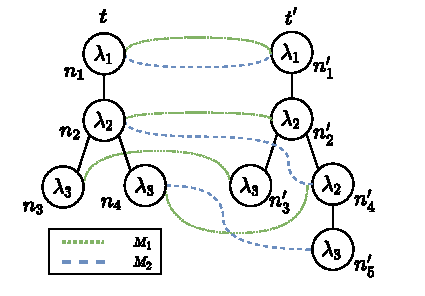
\includegraphics[width=.8\linewidth]{explanation/example_matchings}
    \caption{Illustrating two possible matchings $M_1, M_2$  between two trees $t, t'$. $\lambda_1, \lambda_2, \lambda_3$ are all possible labels for nodes in $t$ and $t'$.}
    \label{fig:tree_matching_example}
\end{figure}

The remainder of this paper is organized as follows.
\Cref{sec:background} introduces the required background and defines the key terms used by the literature.
\Cref{sec:related_work} covers the related work.
\dots
\Cref{sec:conclusion} concludes and overviews some perspectives for this work.



\section{Background \& Definitions}\label{sec:background}
Tree matching refers to the capability of comparing two trees to highlight the changes operated on the source tree in order to build the destination tree.
More formally, we define an ordered tree $t \in T$ as a directed graph $(N,\prec)$ where $N$ is the non-empty set of nodes and $\prec$ a total order relation that can relate a \emph{child} node $c \in N$ to its \emph{parent} $p \in N$, as $c \prec p$, or \emph{siblings}, as $s \in N$, as $c \prec s$.
% a directed relation mapping a \emph{child} node $c \in N$ to its \emph{parent} $p \in N$, as $c \prec p$.

\subsection{Tree Matching}\label{sec:tree_matching}
In 1979, \cite{Tai1979} first mentions and proposes a solution to the problem of comparing two trees.
The problem is formulated as a generalisation of the well studied \emph{string edit distance} and called \emph{Tree Edit Distance} (TED).
Given two labeled trees, $t,t' \in T$, the motivation of TED is to find the least-cost sequence of \emph{edit} operations (relabel, insertion, removal) to transform $t$ into $t'$.
Interestingly, once the sequence of least-cost edit operations is identified, it is possible to extract a \textit{mapping} between the two trees---\emph{i.e.}, the set of couples $(n, n') \in N \times N'$ indicating, for each node $n \in N$, the matching node $n' \in N'$.
In summary, TED algorithms thus compare two trees $t$ and $t'$ by producing
\begin{inparaenum}[\em (a)]
\item a \emph{scalar} $distance(t, t'):(N \times N') \mapsto [0,1]$, and
\item a \emph{node}  $mapping(t, t') \mapsto (N,N')$.
\end{inparaenum}

Despite efforts towards more efficient algorithms~\cite{zhang1995algorithms} and implementations~\cite{Pawlik2011, pawlik2015efficient, pawlik2016tree}, TED remains expansive to compute with---at best---a worst-case time complexity in $O(N^3)$ (where $N$ is the maximum number of nodes in both trees), as recently demonstrated by~\cite{bringmann2018tree}.

It is worth to mention that the scalar distance can help in solving a related problem: \emph{tree similarity join}.
Given a set of $T$ trees, similarity join solutions can cluster similar trees without computing all $|T|^2$ distances between trees~\cite{Guha2002ApproximateJoins,Hutter2019EffectiveJoins,Kailing2004EfficientDatabases,Tang2015ScalingData,Yang2005SimilarityData}.
In order to speedup the comparison of trees, many studies offered restricted versions of TED by trading accuracy for faster computation times~\cite{augsten2008pq,jiang1994alignment,reis2004automatic,selkow1977tree,valiente2001efficient,zhang1995algorithms, zhang1996constrained}.
However, many of these optimizations only compute a distance with no mapping~\cite{augsten2008pq, Wang2001FindingHierarchy, Garofalakis2005XMLEmbeddings}---and thus do not provide solutions to the tree matching problem.
We consider these families of optimizations as out of the scope of this paper.

\vspace{12pt}
\noindent\textbf{Terminologies.}
Formally, a \emph{tree matching} between two labeled trees $t$ and $t'$ is a one-to-one binary relation between a node $n$ of $t$ and a node $n'$ of $t'$: a matching $M$ between $t$ and $t'$ is the set of tuples $M=\{(n,n') \in N \times N'\}$ where any node $n \in N$ matches at most one node $n' \in N'$, and inversely.
For example, we can formally the two mappings of Figure~\ref{fig:tree_matching_example} as:
\begin{equation}
\begin{split}
M_1 & = \{(n_1, n'_1), (n_2, n'_2), (n_3, n'_3), (n_4, n'_4)\} \\
M_2 & = \{(n_1, n'_1), (n_2, n'_4), (n_4, n'_5)\}
\end{split}
\end{equation}

In this paper, we call each pair $m = (n,n') \in M$ a \textit{match} and we note $\lambda(n)$ the label of the node $n$.

As a consequence of TED definition, a \textit{tree mapping} produced by TED is a restricted matching $M_{TED}$ where the ordering of ancestors and siblings must be preserved.
Formally, a matching $M_{TED}$ between $t$ and $t'$ is a \emph{tree mapping} iff, $\forall (n_1, n'_1), (n_2, n'_2) \in M_{TED}$:
\begin{compactenum}
\item $n_1$ is on the left of $n_2$ $\iff$ $n'_1$ is on the left of $n'_2$,
\item $n_1$ is an ancestor of $n_2$ $\iff$ $n'_1$ is an ancestor of $n'_2$.
\end{compactenum}

Then, a \emph{tree alignment} is a further restriction of a mapping where node insertions happen before deletions~\cite{jiang1994alignment}.
Other restrictions exist, like \emph{isolated-subtree mappings}~\cite{TANAKA1988THEPROBLEM}, \emph{top-down mappings}~\cite{Chawathe1999ComparingMemory}
and \emph{bottom-up mappings}~\cite{valiente2001efficient}, which are restricted mappings enabling faster computation times (\emph{e.g.}, a top-down mapping is a mapping where parents of nodes in the mapping must also be in the mapping).
Based on the hierarchy of \cite{valiente2001efficient}, \Cref{fig:hierarchy_matching} summarizes the hierarchy of matchings from the most general to the most restricted (top-down and bottom-up mappings). The bottom-up and top-down mappings intersects when the compared trees are isomorphic (denoted $\cong$).

\begin{figure}
    \centering
    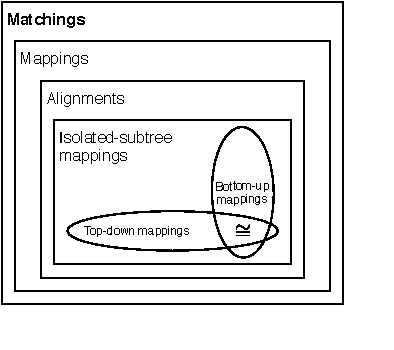
\includegraphics{explanation/hierarchy_matching.pdf}
    \caption{Hierarchy of matchings from the most general to the most restricted}
    \label{fig:hierarchy_matching}
\end{figure}

While TED mappings have received extensive attention, the general tree matching problem remains surprisingly less considered.
In their work on \emph{Flexible Tree Matching} (FTM)~\cite{Kumar2011_FTM}, Kumar~\emph{et~al.} pointed out that the restrictions of TED mappings---\emph{i.e.}, sibling and ancestor order should be preserved---can lead to inaccurate matchings in many cases where the order of siblings and ancestors can change, which is typically the case for phylogenetic trees in biology and DOM trees in web applications.

In the rest of this paper, we therefore address the general problem of tree matching by assuming none of the restrictions imposed by TED and related algorithms.

\subsection{Problem Statement}
A major obstacle to developing new solutions to solve the tree matching problem is the need for a robust way to evaluate and compare solutions.
To the best of our knowledge, at this date, there is no empirical benchmark available to evaluate the \emph{quality} of computed matchings.
Indeed, the literature only focuses on a theoretical analysis of how the proposed solution formally compares to TED (see \Cref{sec:related_work}), but none of the published papers succeeds to deliver a qualitative evaluation of the produced matchings.

This is partly because empirically evaluating the quality of a matching is a complex problem.
Ideally, to evaluate the quality of a matching $M$, we need a baseline, known as the \emph{ideal matching} $M_{ideal}$.
Given $M_{ideal}$, we can compute the
\begin{inparadesc}
    \item[\emph{precision}] as $|M \cap M_{ideal}| / |M|$, and the
    \item[\emph{recall}] as $|M \cap M_{ideal}| / |M_{ideal}|$.
\end{inparadesc}

Unfortunately, providing a wide diversity of ideal matchings is not trivial at scale:
\begin{compactenum}
    \item The most challenging matching problems involve large trees including thousands of nodes.
    On such trees, a human would struggle to even visualize both trees;
    \item In practice, there is often more than a unique "ideal" matching (cf. Figure~\ref{fig:tree_matching_example}).
    The number of "acceptable" matchings tends to grow with the size of the considered trees.
    Asking a single human to manually determine $M_{ideal}$ would inevitably result in biases.
\end{compactenum}

If there is no such thing as an "ideal" matching, then $M_{ideal}$ depends on parameters specified by the user to describe how to match.
For example, TED solutions can tune their matchings by setting three parameters: the \emph{relabel}, \emph{insertion}, and \emph{deletion costs}.
A benchmark to evaluate tree matching solutions should therefore describe the desired matching in a similar way.

In this paper, we report on our solution to the above evaluation challenges.
Our tree matching benchmark, called \forrest, intends to evaluate the \emph{precision} and \emph{recall} of any tree matching without any human supervision.
Then, we apply \forrest to the state-of-the-art implementation of TED on a synthetic dataset in order to evaluate how accurately, \forrest predicts the accuracy of the tree matching solution under study.
And...

\section{Related Work}\label{sec:related_work}
In this section, we describe how solutions to the tree matching problem are being evaluated by the literature.
In most of the seminal papers, no empirical evaluation is reported~\cite{jiang1994alignment,valiente2001efficient,zhang1995algorithms, Dinitz1998OnIsomorphism, Bunke1998ASubgraph, Wang2001FindingHierarchy}.
This is justifiable by the fact that these solutions usually offer strong theoretical bases to the provided algorithms.
However, the absence of empirical evaluation makes it hard to understand how the different algorithms and the trade-offs they adopt impact the performances in practice.

APTED~\cite{pawlik2015efficient, pawlik2016tree}, however, provides a valuable extensive open benchmark for its algorithm, by compiling several open databases of trees.
However, except the Bolzano dataset~\cite{augsten2008pq}, none of these databases are labeled with a ground truth and, when evaluating APTED, only the computation times are reported---which is legitimate in the scope of this paper, since APTED produces an optimal solution to the TED problem.

The Bolzano dataset has been introduced by Augsten~\emph{et~al.}~\cite{augsten2008pq} to link records from two databases of addresses.
To do so, the authors converted each postal address into a tree aggregating some of its characteristics and they used the \emph{pq-Gram} tree distance to compare the address trees.
The algorithm was evaluated against other algorithms by comparing the results with manually labeled record linkages between the two databases: for each address tree in the first database, the corresponding address tree in the second one is assumed to be known.
While this open dataset is helpful to evaluate solutions to the tree similarity join problem---\emph{i.e.}, matching two sets of full trees---it does not contribute to evaluate the finer grained node-to-node matchings between two trees.

Some other works evaluate tree matching solutions on dedicated application domains, like the comparison of waveforms~\cite{Cheng1985WaveformMatching}, RNA structures~\cite{Shapiro1990ComparingComparisons}, a particular use of web page matching like automatic design transfering~\cite{Kumar2011_Bricolage}, or news extraction~\cite{reis2004automatic}.

In conclusion, existing works describing solutions to the tree matching problem do not offer any qualitative benchmark of their algorithm.
This lack of qualitative benchmark makes it hard to:
\begin{inparaenum}
    \item compare different algorithms on realistic datasets, and
    \item develop new algorithms that are not based on TED (and thus cannot formally relate to it).
\end{inparaenum}
To address these limitation, \forrest therefore delivers an open benchmark for the qualitative assessment of tree matching algorithms.

% \section{Tree~Matching Metrics}\label{sec:matching-cost}
% \subsection{Computation Time}
% quality of the implementation?
% \subsection{Matching Quality}
% When perfect matchings are not as obvious as expected, one should therefore tolerate candidate matchings as reasonable solutions.
% To do so, we introduce a new matching metrics that aims to characterize the quality of a tree matching.
% When this metrics equals $1$, a tree matching is then considered as perfect---\emph{i.e.}, all nodes are matched with the best fitting counterpart.
% When this metrics equals $0$, a tree matching is considered as a failure---\emph{i.e.}, none of the nodes succeed to be matched.
% By taking inspiration from pattern recognition, information retrieval and classification domains, we aim to define \emph{precision} and \emph{recall} metrics to capture the quality of a tree matching.

% \section{From Edit To Matching Distance}
% Unlike tree matching, TED aims at identifying the minimal editing distance, which may restrict the associated mappings.
% As explained in \Cref{sec:tree_matching}, the TED between two trees $t$ and $t'$ is defined as the least-cost sequence of elementary operations to transform $t$ into $t'$.
% This means that TED focuses on the costs of edit operations and not the number of operations to perform in order to transform $t$ into $t'$.

% In this section, we adopt a different perspective on this transformation problem by considering the shortest sequence of operations to perform in order to transform $t$ into $t'$.

% In order to transform a tree $t$ into $t'$, we thus apply a sequence of elementary mutations $e \in E$ that conforms to a given matching $M$, which is assumed to be known.
% \begin{defn}
%     Given two trees $t, t'$ and the ideal matching $M$ between the trees, we define the \emph{Shortest Mutation Sequence} (SMS) from $t$ to $t'$ with respect to $M$ and note $SMS(t,t',M) = [e_0, e_1, ..., e_n]$ as the shortest sequence of elementary mutations $e_i \in E$ that transforms $t$ in $t'$ such that each node $n \in N$ is ultimately transformed into $n' \in N'$ iff $(n, n') \in M$.
% \end{defn}

% Given the definition of the \emph{Shortest Mutation Sequence} (SMS), we then define the \emph{Tree Matching Distance} (TMD) as follows.
% \begin{defn}{Tree Matching Distance}
%     Given two trees $t, t'$ and a matching $M$ between $t$ and $t'$, we define the \emph{Tree Matching Distance} (TMD) between $t$ and $t'$ with respect to $M$ and note $TMD(t,t',M)=|SMS(t,t',M)|$ as the length of the shortest mutation sequence between $t$ into $t'$ with respect to $M$.
% \end{defn}

% As mentioned above, TMD differs from TED by focusing on the shortest sequence of mutations to apply, instead of considering the cost of operations.
% From the above, we claim the following theorem:
% \begin{theorem}
%     For all $(t,t',M)$, there exists a shortest mutation sequence (SMS) between $t$ and $t'$ with respect to $M$, where $t, t'$ are trees and $M$ is a matching.
% \end{theorem}

% In order to prove this theorem, we design the following algorithm to compute the shortest mutation sequence between $t$ and $t'$ with respect to $M$, for all $(t, t', M)$.
% This algorithm loops until all nodes of tree $t$ have been visited.
% Whenever a node is visited, the function \emph{mutation} decides the mutation to apply to the input tree $t$, according to the provided matching $M$.
% If a mutation is required, then the current tree is mutated and the ordered list of nodes is updated by traversing the resulting tree in post-order to reflect the change operated in the tree structure.
% When the algorithm completes, all nodes have been visited in post-order traversal that follows the total order $\prec$ (cf. \Cref{alg:sms}).

% \begin{algorithm}
%     \DontPrintSemicolon
%     \SetAlgoLined
%     \KwData{$t$, $t'$, $M$}
%     \KwResult{shortest sequence of elementary mutations}
%     % $M_{copy} \gets$ copy($M$)\;
%     $visited \gets \emptyset$\;
%     $t_{current} \gets copy(t)$\;
%     \While{$|visited| < |nodes(t)|$}{
%         $N \gets postOrder(t_{current})\setminus visited$ \;
%         \For{$n \in N$}{
%             $visited \gets visited \cup n$\;
%             $m \gets mutation(n, M)$ \;
%             \If{m $\neq \varnothing$}{
%                 $t_{current} \gets m(t_{current})$ \;
%                 \Break \;
%             }
%         }
%     } % The following part is not described in text.
%     \For{n' $\in leaves(t')$}{
%         $N \gets []$ \;
%         $P \gets n'$\;
%         \While{$M^{-1}(P) = \varnothing$}{
%             $N \gets N \cup P$\;
%             $P \gets parent(P)$\;
%         }
%         \For{$n \in reverse(N)$}{
%             Add($t$,n,$M^{-1}$(P)) \;
%             \tcp{n is a leaf node (not a subtree)}
%         }
%     }% The returned value is missing... how do you prove this is the SHORTEST sequence?
%     \caption{Shortest Mutation Sequence}\label{alg:sms}
% \end{algorithm}

% Then, the set of elementary mutations $e \in E$ returned by the function $mutation$ requires to be enumerated.
% When looking more closely t o the possible situations faced by \Cref{alg:sms}, we observe the following cases when traversing the input tree $t$ in a post-order:
% \begin{compactenum}
%     \item the leaf node $n'$ is does not appear in the matching $M$, which means that it should be \emph{inserted},
%     \item the leaf node $n$ is associated to a different parent in $t'$, which means that it should be \emph{moved},
%     \item the leaf node $n$ is associated to the same parent in $t$, but with a different label, which means that it should be \emph{relabelled},
%     \item the leaf node $n$ does not appear in the matching $M$, which means that it should be \emph{deleted}.
% \end{compactenum}

% From this observation, we define the set of elementary mutations $E$ as follows:
% \begin{defn}
% An elementary mutation is a function $e: T \mapsto T'$ that transforms a tree $t$ into another tree $t'$ by applying one of the following functions:
% \begin{compactitem}
%     \item $ins(t,l,a)$ builds a tree $t'$ by inserting the leaf node $l$ as a child of $a$ in $t$ according to the ordering relation $\prec$,
%     \item $mov(t,a,b)$ returns a tree $t'$ by replacing the current parent of any node $a$ in $t$ by $b$ (hence moving the subtree rooted in $a$) and respecting the ordering relation $\prec$,
%     \item $rel(t,a,\lambda)$ outputs a tree $t'$ by relabelling any node $a$ in $t$ to $\lambda$,
%     \item $del(t,l)$ produces a tree $t'$ by removing the leaf node $l$ from $t$.
% \end{compactitem}
% where $a, b$ are any nodes of $t$, $l$ is a leaf node of $t$ and $\lambda$ is a label.
% \end{defn}

% \begin{prop}
%     Given a tree $t$, an elementary mutation $e \in E$ changes the ancestry and/or the label of at most one node $n$ in $t$.
% \end{prop}
% The proof is trivial when looking at the definition of each elementary operation.
% So what... what is the conclusion here?

% Table with the mapping/differences between TED operations and TMD mutations.

%  Take care of the transition with the following section
\section{FORREST Benchmark Suite}\label{sec:forrest}
The \forrest benchmark suite intends to evaluate the quality of tree matching algorithms on a wide diversity of trees without requiring manual labeling.
To do so, \forrest leverages two complementary approaches:
\begin{compactenum}
    \item A \emph{synthetic benchmark} that uses mutation-based dataset obtained by mutating a set of reference trees while keeping track of the ground truth (\emph{i.e.}, ideal matching);
    \item A \emph{realistic benchmark} that can be applied when the ground truth is not known but requires the tuning of a parameter;
\end{compactenum}

Both approaches provide a complementary perspective on the qualitative evaluation of tree matching algorithms.
% The synthetic benchmark allows to evaluate any tree matching solution in a controlled environment. 
% In particular, since all mutations applied are known, it allows a fine-grained analysis of the sensitivity of the matching algorithms to each type of mutations.
By using this benchmark suite, the research community can identify the strengths and weaknesses of existing tree matching algorithms in order to identify the properties of trees that make their matchings more or less accurate.
We also believe that the adoption of this benchmark suite can contribute to the emergence and robust assessment of new tree matching algorithms for which purely theoretical evaluation is particularly challenging.

\subsection{Benchmark Metrics}
Given $|M|$ and $|M_{ideal}|$ the set of matchings reported by the algorithm and the ground truth, respectively, one can define the benchmark metrics as follows:
\begin{equation}
    precision(M) = \frac{|M \cap M_{ideal}|}{|M|}
\end{equation}
that reflects the rate of true positives over the set of predicted matchings, and:
\begin{equation}
    recall(M) = \frac{|M \cap M_{ideal}|}{|M_{ideal}|}
\end{equation}
that denotes the rate of true positives over the set of actual positive matchings.
Based on these two metrics, one can also compute the aggregate $f1$ score, balancing $precision$ and $recall$, as:
\begin{equation}
    f1(M) =  2 \times \frac{precision(M) \times recall(M)}{precision(M) + recall(M)} 
\end{equation}


\subsection{Mutation Dataset}\label{sec:mutation}
The mutation dataset provides a trustworthy estimation of the quality of tree matching algorithms over sample trees that are synthetically mutated.
In the mutation dataset we describe below, the ground truth (ideal matching) is always known.
Using such a dataset thus allows \forrest{} to compute the precision and recall of any tree matching algorithms on potentially very large datasets of trees.

Synthetic datasets are commonly used to evaluate (usually the computation times of) TED-related algorithms~\cite{XXX}.
However, to the best of our knowledge, no existing approach synthetically builds a dataset where the fine-grained node-to-node matching is known.

The idea of our approach is the following.
For each tree $t$ in a set of source trees $T_{source}$:
\begin{compactenum}
    \item Mark every node $n$ in $t$ with a unique \textit{signature} $s \in S$,
    \item Apply a given number of mutations to $t$ thus transforming $t$ into $t'$,
    \item Use the signatures $S$ to find the ideal matching $M$ between $t$ and $t'$,
    % \item Replace all the signatures $S$ in $t'$ by a unique signature $s' \in S'$ and update the ideal matching accordingly, as pairs defined as $(S) \mapsto S'$, thus avoiding any matching bias exploiting a common signature.
\end{compactenum}

More precisely, our algorithm that generates the synthetic dataset can be tuned with the following parameters:
\begin{compactenum}
	\item $r_{max}$: the maximum mutation ratio to be applied on an source tree $t$,
    \item $n_{mutants}$: the number of mutant trees $t'$ to generate for each given source tree $t \in T_{source}$,
    \item  $mutate(t,r):(T\times[0,1])\mapsto T \times (N \times N')$: the mutation function that takes any tree $t$ as an input and applies a given ratio of random mutations $r$ to produce a mutated tree $t'$, together with the ideal matching $M$ between the input tree $t$ and the mutated tree $t'$.
\end{compactenum}
For each tree $t \in T_{source}$, the function $mutate$ is called $n_{mutants}$ times for a ratio randomly chosen between $0$ and $r_{max}$.
The resulting synthetic dataset contains $|T_{source}|$.

% The mutation algorithm is implemented as follow:
% \begin{algorithm}
% \DontPrintSemicolon
%     \SetAlgoLined
%     \KwData{$t$, $r$}
%     \KwResult{mutated tree $t'$}
%     nodes $\gets$ shuffle($t$.nodes)\;
%     nbNodesToMutate $\gets$ $r \times$ nodes.count()\;
%     mutations $\gets$ []\;
%     \While{nbMutations < nbNodesToMutate}{
%         mutationType $\gets$ getRandomMutationType()\;
%         node $\gets$ nodes.pop()\;
%         mutations += apply(mutationType, node))\;
%     }
% \nd{algorithm}

The most challenging part of the above approach is to write the function $mutate$ by considering the appropriate set of mutations to apply to $t$ in order to generate mutants that are representative of real-life mutations.

While writing a generic $mutate$ function that applies to any tree is technically feasible, there is no guarantee that these mutations will reflect the mutations happening in a given class of trees.
For example, when comparing two syntax trees to display a diff between two code versions, a tree matching algorithm should be tuned with mutations that refer to common code refactorings.

This is why we chose to leave the definition of the function $mutate$ as a parameter of our approach, which depends on the domain understudy. 
In \Cref{sec:application}, we describe an example of mutation strategy for the specific case of DOM tree matching.

\subsection{The Realistic Benchmark}\label{sec:forrest_accuracy}
The \forrest accuracy approximates the precision and recall metrics for a given matching $M$ between two trees $t$ and $t'$.

\subsubsection{Tree Matching Precision}
The precision of a matching is defined as the ratio of correct matches over the total number of identified matches: $precision(M)=|correct(M)|/|M|$.

Let us define the following matching accuracy function:
\begin{equation}
accuracy(m) =
\begin{cases}
    1 &\text{if the match } m \text{ is correct},\\
    0 & \text{otherwise}
\end{cases}
\end{equation}
Where the pair $m=(n, n') \in M$ is a match.
Then, we can define the $precision$ of a matching $M$ as:
\begin{equation}
    precision(M) = \frac{1}{|M|}\sum_{m \in M}accuracy(m)
\end{equation}

Since we usually do not have access to the above defined $accuracy$ function, our purpose is to propose an estimated accuracy function $\hat{accuracy}$ allowing us to compute an approximated precision $\hat{precision}$.

To do so, we consider the cost function described in the \emph{Flexible Tree Matching} (FTM)~\cite{Kumar2011_FTM}.
In their work, Kumar~\emph{et~al.} use an approximation of this cost to compute a matching between two trees, as using the exact cost would be too expensive to compute. 
The cost we introduce here is a modified version of the FTM cost that we use, instead, to evaluate a reported matching.

Let us consider a match $m=(n, n') \in M$ where $n$ is a node of $t$ and $n'$ is a node of $t'$.
We define $c(m):(N \times N') \to [0, 1]$ as the cost of a matching $m$, computed as:
\begin{equation}\label{eq:FTM_cost}
% \begin{aligned}
    c(m) = w_r \cdot c_r(m) + w_a \cdot c_a(m) + w_s \cdot c_s(m)
% \end{aligned}
\end{equation} 
where $c_r, c_a, c_s$ are the relabeling, ancestry and sibling costs, respectively, and $w_r, w_a, w_s$ are associated weights, such that $w_r + w_a + w_s = 1$.

In order to define the relabel, ancestry and sibling costs, we adopt the following notations:
\begin{compactitem}
\item $S(n)$ and $C(n)$ are the sets of siblings and children of a node $n$, respectively.

\item Given a matching $M$ and $O \subseteq N$ or $O'\subseteq N'$, we note $M(O) = \{n \in O | (n, n') \in M, n' \in N'\}$ the image of $O$ by the matching $M$ and inversely, $M^{-1}(O') = \{n' \in O' | (n',n), n \in N\}$ (\emph{e.g.}, if nodes $n_1, n_2$ match with $n'_1, n'_2$, then $M(\{n_1, n_2\}) = \{n'_1, n'_2\}$ and $M^{-1}(\{n'_1, n'_2\}) = \{n_1, n_2\}$).

\item $A \bigtriangleup B$ is the disjunctive union between the sets $A$ and $B$---\emph{i.e.}, the set of elements in $A \cup B$ either of the sets and not in their intersection.

% \item $d_J(A, B) = (|A \cup B| - |A \cap B|) / |A \cup B|$ is the Jaccard distance measuring the ratio of different elements in sets $A$ and $B$.
\end{compactitem}

For a given match $m=(n,n') \in M$, we define the three costs as follow:
\begin{compactenum}
    \item The \textbf{relabel cost} estimates the cost for editing two labels.
    For example, in \Cref{sec:evaluation}, we consider the Jaccard distance ($d_J$) between labels $\lambda(n)$ and $\lambda(n')$:
    \begin{equation}
        c_r = d_J(\lambda(n), \lambda(n')) = \frac{|tk(n) \bigtriangleup tk(n')|}{|tk(n) \cup tk(n')|}
    \end{equation}
    where $tk(n)$ is the set of tokens in $\lambda(n)$;

    \item As an intermediary function to express the two remaining costs, we define the \textit{violation ratio} $v$ between $O \subset N$ and $O' \subset N'$:
    \begin{equation}
        v(O, O') = \frac{|M(O) \bigtriangleup O'| + |O \bigtriangleup M^{-1}(O')|}{|M(O) \cup O'| + |O \cup M^{-1}(O')|}
    \end{equation};
    
    \item The \textbf{ancestry cost} can be defined as follows:
    \begin{equation}
        c_a = v(C(n), C(n'))
    \end{equation}
    where the \textbf{ancestry cost} penalizes the match $(n,n')$ if the children of $n$ are not matched with the children of $n'$, and inversely;

    \item Finally, following the same idea, the \textbf{sibling cost} penalizes the match $(n, n')$ if the siblings of $n$ are not matched with the siblings of $n'$, and inversely:
    \begin{equation}
        c_s = v(S(n), S(n'))
    \end{equation}
    since $\forall (A, B), A \bigtriangleup B \leq A \cup B \implies v(A, B) \leq 1$, which means that, for all matchings $M$, $c(M) \leq 1$.
\end{compactenum}

For each match $m = (n, n')$, we then use the matching cost $c(m)$ to decide whether the match is correct or not.
This can be seen as a binary classification with only one feature (the matching cost). 
For the decision, we use a simple threshold $\tau$, which yields the following formula for the estimated accuracy $\hat{accuracy}$:
\begin{equation}
\hat{accuracy}(m) = 
\begin{cases}
   1 & \text{if } c(m) < \tau \\
   0 & \text{otherwise}
\end{cases}
\end{equation}

In order to determine $\tau$, we need to use a dataset of matchings $\mathscr{M}$ where the ground truth is known, like the mutation dataset (cf. \Cref{sec:mutation}).
Then, $\tau$ is chosen to minimize the approximation error of $\hat{accuracy}$:
\begin{equation}
  \tau = \argmin_{\tau \in [0, 1]}\sum_{M \in \mathscr{M}}|\hat{accuracy}(M) - accuracy(M)|
\end{equation}

Finally, this accuracy estimate is used to compute an approximation of the precision:
\begin{equation}
    \hat{precision}(M) = \frac{1}{|M|}\sum_{p \in M}\hat{accuracy}(p) \\
\end{equation}

\subsubsection{Tree Matching Recall}
The recall of a matching measures the ratio of correct matches in $M$ over the total number of correct matches in $M_{ideal}$:
\begin{equation}
    recall(M) = \frac{1}{|M_{ideal}|} \sum_{m \in M} accuracy(m)
\end{equation}
Since we already described a way to compute an approximate $\hat{accuracy}$ of accuracy, we now need to find a way to approximate $|M_{ideal}|$.
Given two trees $t$ and $t'$, the ideal matching $|M_{ideal}|$ represents the number of all possible correct matches.
If $t$ and $t'$ have the same number of nodes and each node in $t$ matches with a node in $t'$ then $|M_{ideal}| = |N| = |N'|$.
However, in the general case, there can be deletions and insertions between $t$ and $t'$. 
In this case, the inserted and deleted nodes do not appear in $M_{ideal}$.
In order to approach $|M_{ideal}|$, we use $min(|N|,|N'|)$ as an upper bound of $|M_{ideal}|$.
Since $|M_{ideal}| \leq min(|N|, |N'|)$, we have the following lower bound for $recall(M)$:
\begin{equation}
    recall(M) \geq \frac{1}{min(|N|, |N'|)} \sum_{m \in M} accuracy(m)
\end{equation}
when the compared trees are similar (\emph{e.g.}, for change tracking), or when one of the trees is a small pattern where most nodes are expected to be matched, this lower bound is a good approximation of the underlying recall.
When both trees are large and mostly unrelated, the lower bound may underestimate the true recall.

Our final formula for $\hat{recall}(M)$ using the previously described accuracy estimates $\hat{accuracy}$ is the following:
\begin{equation}
    \hat{recall}(M) = \frac{1}{min(|N|, |N'|)} \sum_{m \in M} \hat{accuracy}(m)
\end{equation}
Similarly to $\hat{precision}$ we can define $\hat{recall}_c$ using $\hat{accuracy}_c$.

\section{Application to TED on Webpages\label{sec:application}}
In this section, we apply \forrest to evaluate the quality of TED mappings on a dataset of synthetically mutated webpage DOM trees.
This section has two goals:
\begin{compactenum}
	\item Evaluate the accuracy of \forrest when estimating the precision and recall of mapping $M_{TED}$ produced by TED.
	\item Provide a concrete example of applications for \forrest.
\end{compactenum}
We do not aim to provide an exhaustive comparative benchmark of TED solutions.

\subsection{Webpage Synthetic Dataset}
\paragraph*{Methodology}
A mutation-based synthetic dataset can evaluate matchings in a controlled environment where the ground-truth is known.

We apply the algorithm described in \Cref{sec:mutation} to the specific example of webpage DOM trees.

The algorithm mainly requires to provide a function $mutate: (T \times [0, 1]) \to (T, M)$ that takes a tree $t$ and a mutation ratio $r$ as input and returns a mutated tree along with the ideal matching $M$.

As mentioned in \Cref{sec:mutation}, the $mutate$ function highly depends on the domain understudy. 
In our case, we consider webpage DOM trees.
The DOM (\emph{document object model}) of a webpage is the structure used internally by browsers to represent a webpage (after parsing the HTML content of the page).
Comparing different versions of a webpage DOM is a common problem~\cite{XXX} and can be achieved using tree matching algorithms~\cite{XXX}.

In a DOM tree, most nodes are HTML elements whose labels consist in:
\begin{inparaenum}
    \item a tag name (\emph{e.g.}, \texttt{a}, \texttt{h1}, \texttt{head}),
    \item a list of attributes (\emph{e.g.}, \texttt{class}, \texttt{id}, \texttt{href}) along with their value,
    \item the raw content of the HTML element 
\end{inparaenum}

In order to create the $mutate$ function, we interviewed experienced web developers who reported on the most common mutations between different versions of the same page.
Following their inputs, we compiled the following list of possible mutations:
\begin{center}
  \begin{tabular}{|l l|} 
      \hline
      Node          & Mutation operators\\
      \hline
      \hline
      \em Structure & \tt remove, duplicate, wrap, unwrap, swap \\
      \em Attribute & \tt remove, remove words \\
      \em Content   & \tt replace with random text, \\
                    & \tt change letters, remove, remove words \\
      \hline
  \end{tabular}
\end{center}

Where
\textit{Structure: remove} removes an element and its children (recursively), 
\textit{duplicate} duplicates a subtree, applies $mutate$ to duplicated subtree and insert the subtree anywhere in the tree,
\textit{wrap} wraps an element within a new $div$ container,
\textit{unwrap} removes an element $e$ and attach the children of $e$ to the parent of $e$,
\textit{swap} swaps the position of two sibling elements,
\textit{Attribute: remove} removes an attribute with its value,
\textit{Attribute: remove words} removes a random number of tokens from the value of an attribute,
\textit{Content: replace with random text} replaces the content of an element with a random text whose size is close to the original,
\textit{Content: change letters} replaces a few letters in the content of an element,
\textit{Content: remove} removes the content of an element,
\textit{Content: remove words} removes random tokens from the content of an element.


\paragraph{Dataset description}
Using the algorithm described in \Cref{sec:mutation} and the $mutate$ function described above, we computed a dataset of tuples $(t, t', M)$ where $t$ is an original webpage DOM tree, $t'$ a mutant of $t$ and $M$ the ideal matching between $t$ and $t'$ (known because the mutations are tracked).
We used a maximum mutation ratio $r_{max} = 0.5$ and for each original webpage tree $t$, we generated $n_{mutants}=10$.
For the original webpage source $T_{source}$, we used the Top\,1k Alexa, which lists the most visited websites, thus providing a wide variety of real-life webpage DOM trees.
On the obtained mutation dataset, we ran the the APTED implementation of TED~\cite{pawlik2016tree} to produce a mapping for each tuple.
APTED is the state-of-the-art implementation of TED allowing to  effectively compute the optimal TED mapping.
The resulting dataset $\mathscr{M}$ thus comprises a list of tuples $(t, t', M) \in \mathscr{M}$ where $M$ is the TED mapping between the original webpage tree $t$ and its mutation $t'$.

The following table summarizes the key indicators about the dataset $\mathscr{M}$:
\begin{table}[h]
\centering
\begin{tabular}{l|l|ll}
\cline{2-2}
                                           & Web Dataset  &  &  \\ 
\cline{1-2}
\multicolumn{1}{|l|}{\# Tuples}            &        3,385 &  &  \\
\multicolumn{1}{|l|}{\# Matches}           &    1,435,905 &  &  \\
\multicolumn{1}{|l|}{\# Unique URLs}       &          345 &  &  \\
\multicolumn{1}{|l|}{\# Mutations applied} &      568,912 &  &  \\ 
\cline{1-2}
\end{tabular}
\end{table}
For each tuple $(t, t', M) \in \mathscr{M}$, the number of \textit{match} is the number of individual node-to-node association---\emph{i.e.}, $|M|$. The number of \textit{match} is relevant as the accuracy is evaluated at the node-to-node match level.

\begin{figure}
    \centering
    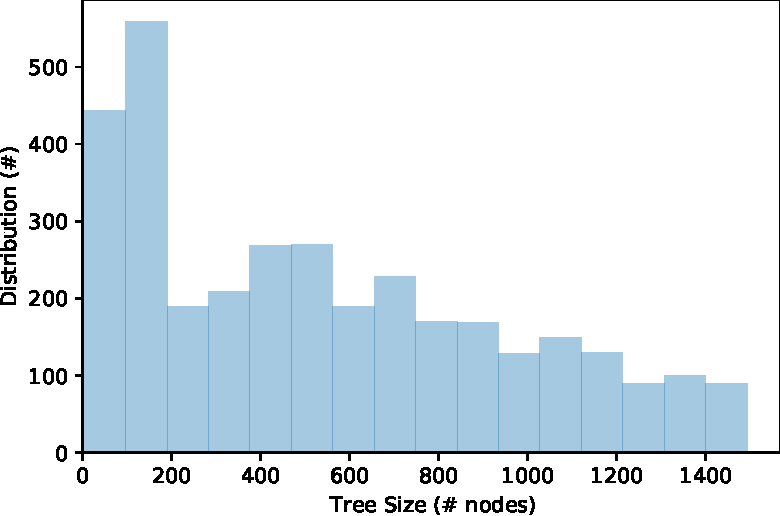
\includegraphics[width=\linewidth]{graphs/tree_size_distribution}
    \caption{Distribution of tree sizes (number of nodes) in the mutation dataset}
    \label{fig:distribution_size}
\end{figure}

\Cref{fig:distribution_size} shows the distribution of tree sizes in the dataset.
We purposely limited the size of the input trees to $1,500$ nodes in order to limit the computation time of the tree matching algorithm APTED whose worst-time complexity is cubic with the number of nodes.

\begin{figure}
    \centering
    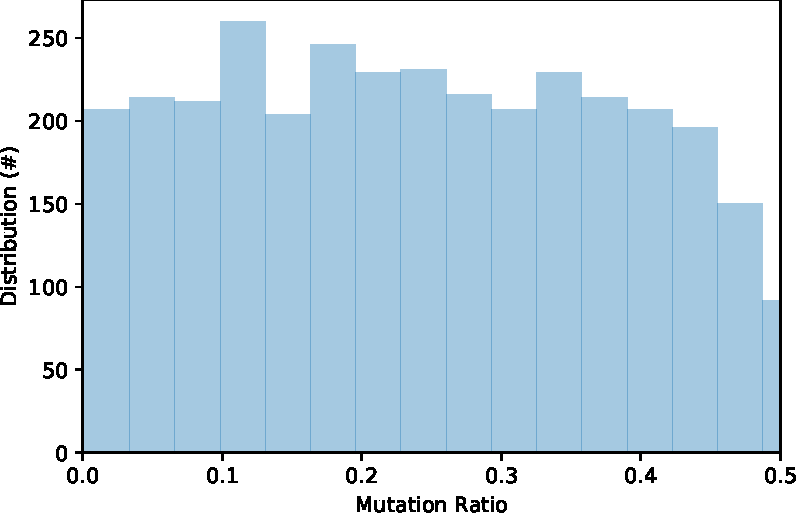
\includegraphics[width=\linewidth]{graphs/mutation_ratio_distribution}
    \caption{Distribution of the applied mutation ratios in the mutation dataset}
    \label{fig:distribution_mutation_ratio}
\end{figure}

Finally, \Cref{fig:distribution_mutation_ratio} describes the distribution of mutation ratios applied to the original webpage DOM trees when building the mutation dataset.


\subsection{Application \& Evaluation of FORREST}
We apply the FORREST benchmark to the previously described mutation dataset.
For each tuple $(t, t', M) \in \mathscr{M}$, we evaluate the precision and recall of the matching $M$ between the trees $t$ and $t'$. 
By doing so, we
\begin{inparaenum}
    \item provide an example of application for FORREST, and
    \item evaluate how accurately FORREST manages to compute the precision and recall on the mutation dataset (where the ground-truth ideal matching is known)
\end{inparaenum}
 
\subsubsection{Ground Truth}

\begin{figure}
     \centering
     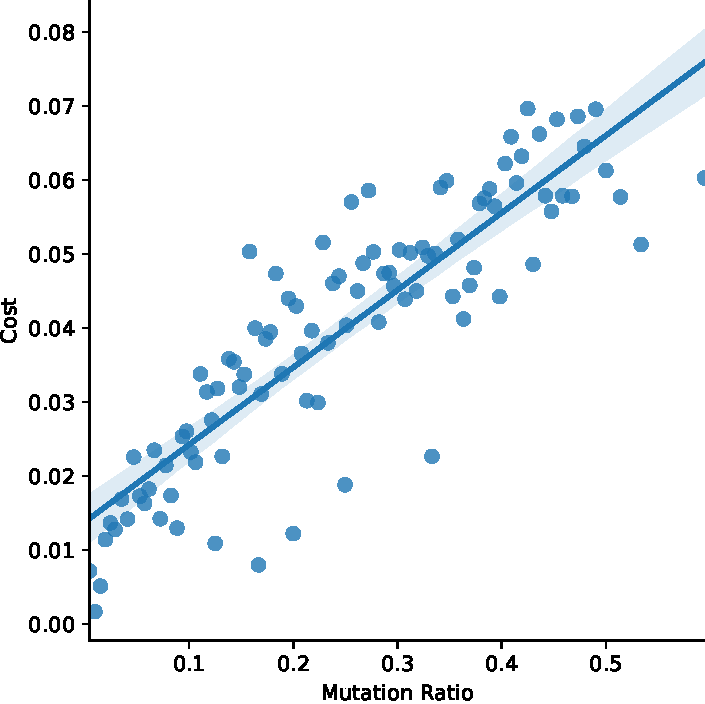
\includegraphics[width=\linewidth]{graphs/mutation_ratio_cost}
     \caption{Evolution of the matching costs when the mutation ratio increases.}
     \label{fig:mutation_ratio_vs_cost}
\end{figure}

In itself, the mutation dataset allows to already measure the quality of matching algorithms on a synthetic dataset.
Figure \ref{fig:mutation_ratio_vs_cost} shows the evolution of matching costs with the mutation ratio.

\subsubsection{\forrest Accuracy Metrics}
We evaluate the ability of \forrest to accurately estimate the precision and recall of a given tree matching algorithm.
In order to do so, we report on the precision and recall of \forrest itself, which is not to be mistaken with the precision and recall of the matching algorithm.
From now, we subscript the metrics with either $f$ or $TED$ when referring to \forrest or the matching algorithm (\emph{Tree Edit Distance} in our case): $precision_{TED}$ and $recall_{TED}$ describe the accuracy of TED matching between two trees while $prevision_f$ and $recall_f$ describe the accuracy of \forrest.

We describe the accuracy of \forrest on a matching $M$ using the ground truth $accuracy$ function and the estimated $\hat{accuracy}$ function described in \ref{sec:forrest_accuracy}.
The confusion matrix \Cref{tab:precision_recall} helps in introducing \forrest's formulas of precision and recall using these accuracy functions.
\begin{table}[h]
    \centering
    \caption{Confusion matrix of \forrest}
    \label{tab:precision_recall}
    \begin{tabular}{|c||*{5}{c|}}\hline
        \backslashbox{$\hat{acc}(m)$}{$acc(m)$}
        &\makebox[3em]{\tt 0}&\makebox[3em]{\tt 1} \\\hline\hline
        \tt 0 & True Negative & False Negative \\\hline
        \tt 1 & False Positive & True Positive \\\hline
    \end{tabular}
\end{table}

Formally, for any matching $M$, we define the following subsets:
\begin{equation}
    \begin{split}
        TP(M) & = \{m | acc(m) = \hat{acc}(m) = 1, m\in M\} \\
        P(M)  & = \{m | acc(m) = 1, m\in M\} \\
        FP(M) & = \{m | acc(m) = 0, \hat{acc}(m) = 1, m\in M\}
    \end{split}
\end{equation}

Using the above subsets allows us to define the precision and recall of \forrest for any matching $M$:
\begin{equation}
    \begin{split}
        precision_f & = \frac{|TP|}{|FP| + |TP|}\\ 
        recall_f    & = \frac{|TP|}{|P|}\\ 
    \end{split}
\end{equation}

\subsubsection{Tuning}
% We divide our dataset $\mathscr{M}$ into two:
% \begin{compactenum}
%     \item $\mathscr{M}_{tr}$: the training dataset ($70\%$)
%     \item $\mathscr{M}_{te}$: the testing dataset ($30\%$)
% \end{compactenum}

% The tuning described below is done on the training dataset while the results presented in section \ref{sec:results} have been computed on the testing dataset.

The precision and recall depend on the $\hat{acc}$ function, whose behavior is determined by the threshold $\tau$ which is the only parameter of the \forrest benchmark.

\begin{figure}
    \centering
    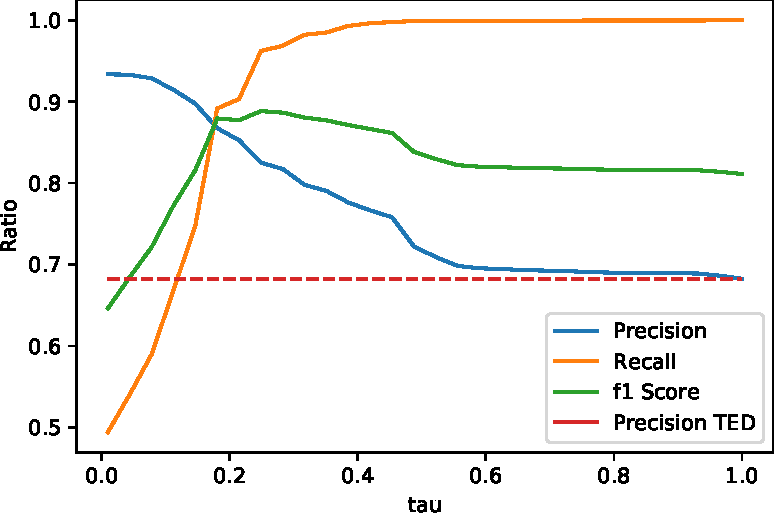
\includegraphics[width=1\linewidth]{graphs/precisionrecall_tau.pdf}
    \caption{Precision and Recall of \forrest according to the parameter $\tau$}
    \label{fig:tuning_tau}
\end{figure}

\Cref{fig:tuning_tau} reports on $precision_f$, $recall_f$ and $f1_f$ according to the parameter $\tau$.
The best value for $\tau$ (the value that maximizes $f1$) yields the following results:
\begin{compactitem}
    \item $precision_f = 0.85$ 
    \item $recall_f = 0.90$ 
    \item $f1_f = 0.87$ 
\end{compactitem}
Interestingly, the lowest possible value for $precision_f$ is $precision_{TED}$.
Indeed, $tau = 1$ implies that $\forall m \in M, \hat{acc}(m) = 1$---\emph{i.e.}, all matches from $M$ are considered accurate which means that the resulting precision is the precision of the matching algorithm that produced $M$.

In addition to allowing to evaluate the matching precision (cf. \Cref{sec:results}), it is also possible to use this approach to improve the results of any matching algorithms.
The matching cost then acts as a confidence metrics and if combined with the threshold-based classification, allows to disqualify matches with a high cost.
\Cref{fig:tuning_tau} shows the ratio of incorrectly disqualified matches ($recall_f$) when trying to improve the precision ($precision_f$) by decreasing $\tau$.
For the optimal value of $\tau$, using the \forrest approach in this manner thus allows us to improve the precision of the algorithm from 68\% to 85\% while reducing the recall by only 10\% which corresponds to an overall gain of 6\% on the $f1$ score.

\subsubsection{Results}\label{sec:results}
The main purpose of \forrest is to evaluate the accuracy of any matching algorithm on datasets where the ground truth ideal matching is unknown.
We are thus interested in studying how close the accuracy estimated by \forrest is compared to the real accuracy on the mutation-based dataset $\mathscr{M}$.

\begin{figure}
    \centering
    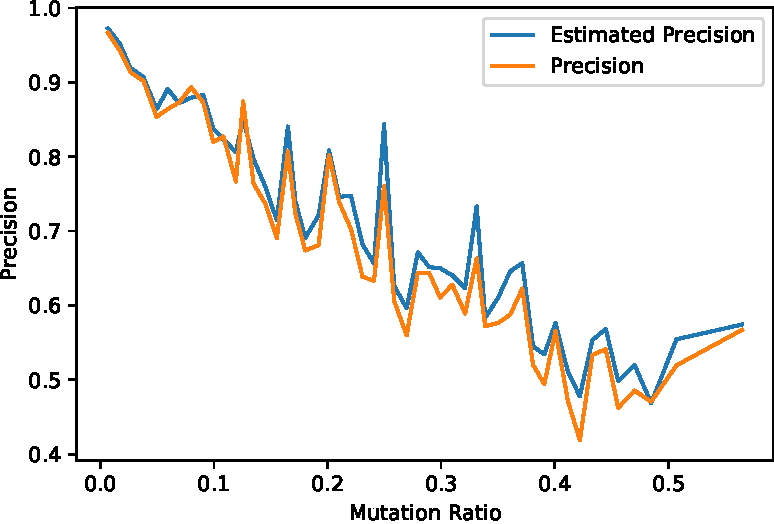
\includegraphics[width=\linewidth]{graphs/estimated_precision_vs_precision}
    \caption{Estimated precision and actual precision according to the mutation ratio.}
    \label{fig:estimate_vs_real_mutation_ratio}
\end{figure}

\Cref{fig:estimate_vs_real_mutation_ratio} depicts how the estimated and actual precision of TED evolves with the mutation ratio.
Given a matching $M$, we define the estimation error of \forrest by: $\epsilon_M = |precision(M) - \hat{precision}(M)|$.
Then, the mean error of \forrest on our dataset is $\epsilon = 7.5\%$.
Concretely, it means any comparison between two tree matching solutions using \forrest could only be conclusive if the comparison shows a gap superior to $\epsilon = 7.5\%$.


\section{Conclusion \& Perspectives}\label{sec:conclusion}
Comparing modern real-life web documents is a challenge for which traditional \emph{Tree Edit Distance} (TED) solutions are too restricted and computationally expensive. 
\cite{Kumar2011_FTM} introduced \emph{Flexible Tree Matching} (FTM) to offer a restriction-free matching, but at the cost of prohibitive computational times.
In this paper, we presented \emph{Similarity-based Flexible Tree Matching} (SFTM), which extends FTM to offer tractable computational times while offering non-restricted matching.
We evaluated our solution using mutations on real-life documents and we showed that SFTM qualitatively compares to TED while improving the performances by two orders of magnitude.
The proof of concept we deliver demonstrates that matching real-life web documents in practical time is possible.

We believe that having a robust algorithm to efficiently compare web documents will open up new perspectives within the web community.
In future work, we will further investigate on how to improve the quality of the matchings by analyzing which situations cause SFTM to make mistakes in order to establish guidelines to adjust the exposed parameters.

Whether our work might be applicable to other trees than web DOMs remains to be tested.
Indeed, SFTM strongly relies on the fact that node labels in DOMs are highly differentiating (many specific attributes on each element), which is not the case for all kinds of trees.

\bibliographystyle{abbrv}
\bibliography{references,references_mendeley}

\end{document}

%%e.g: Given an element $E$ to locate,  $P$ is an ancestor of $E$, if $P$ has differentiating attributes (like an \textit{id}) we can locate $E$ relatively to $P$ and identify $P$ using its differentiating attributes. 

%\subsubsection{Stateful identification architecture}
%Existing methods to identify elements on a page (xPath) are limited. Notably, they don't allow to express \textit{flexible}, statistics based identifiers. That's why some works have developed some more flexible identification methods [...] and applied them to repair broken locators.

%If we are capable to use more efficient methods than xPath to identify elements as these studies suggest, why use it only to repair locators and not directly as locators?

%In this contribution, we study the problems that moving to such a flexible identification system might rise and suggest a possible architecture allowing to practically use \textit{stateful identification methods}.




% A naive approach would be to sort all edges by increasing cost and select $min(|U|, |V|)$ edges.
% However, doing so would not guarantee to obtain a full matching, since we might have selected several edges linked to the same nodes.
% A valid approach would rather be to: 
% \begin{compactenum}
%     \item Sort all the edges by increasing cost,
%     \item Select the edge $e$ between $u$ and $v$,
%     \item In the ordered list, remove all edges other than $e$ linked to $u$ and $v$,
%     \item Repeat the selection process (from step (2)) until all edges have been selected/
% \end{compactenum}

% While this approach returns a full matching, it only optimizes the decision one-step-ahead.
% In order to approach the optimal matching, we use the same technique as FTM does: the metropolis algorithm~\cite{metropolis1953equation}.
% The metropolis algorithm provides a way to explore a probability distribution by random walking through samples.
% We use this algorithm to random walk through several full matching, and retain the least costly.
% The algorithm needs to be provided with:
% \begin{compactenum}
%     \item An initial sample $M_0$,
%     \item A suggestion function $suggestMatching: M_t \mapsto M_{t+1}$,
%     \item An objective function we want to maximize: $f(M)$,
%     \item A parameter $N$ that defines the number of random walk to perform before returning the best visited sample.
% \end{compactenum}
% Table~\ref{tab:equivalenceMetropolis} shows the equivalence between the general vocabulary and notations commonly used when describing the metropolis algorithm and our specific application to FTM.


% \begin{table}
% \caption{Equivalence between the Metropolis algorithm and FTM}
% \label{tab:equivalenceMetropolis}
% \begin{tabular}{ll}
% \hline
% Metropolis Algorithm & FTM                                    \\
% \hline
% Sample $x$           & Full matching $M$                      \\
% $Q(x_{t+1}|x_t)$     & $suggestMatching: M_t \mapsto M_{t+1}$ \\
% Probability distribution $P(x)$ & $f: M \mapsto \text{quality of } M)$ \\
% \hline
% \end{tabular}
% \end{table}
